\documentclass{article}

% if you need to pass options to natbib, use, e.g.:
% \PassOptionsToPackage{numbers, compress}{natbib}
% before loading nips_2017
%
% to avoid loading the natbib package, add option nonatbib:
% \usepackage[nonatbib]{nips_2017}

\usepackage{nips_2017}

% to compile a camera-ready version, add the [final] option, e.g.:
% \usepackage[final]{nips_2017}

\usepackage{polski}
\usepackage[utf8]{inputenc} % allow utf-8 input
\usepackage[T1]{fontenc}    % use 8-bit T1 fonts
\usepackage{hyperref}       % hyperlinks
\usepackage{url}            % simple URL typesetting
\usepackage{booktabs}       % professional-quality tables
\usepackage{amsfonts}       % blackboard math symbols
\usepackage{nicefrac}       % compact symbols for 1/2, etc.
\usepackage{microtype}      % microtypography

\title{Głęboka sieć wielowarstwowa typu MLP}

% The \author macro works with any number of authors. There are two
% commands used to separate the names and addresses of multiple
% authors: \And and \AND.
%
% Using \And between authors leaves it to LaTeX to determine where to
% break the lines. Using \AND forces a line break at that point. So,
% if LaTeX puts 3 of 4 authors names on the first line, and the last
% on the second line, try using \AND instead of \And before the third
% author name.

\author{Karol Kowalski}

\begin{document}
% \nipsfinalcopy is no longer used

\maketitle

\begin{abstract}
  W niniejszej pracy opiszę krótko czym jest sieć wielowarstwowa
  typu MLP oraz przedstawie badania na zbiorze CIFAR.
  Sieć ta składa się z kilku warstw perceptronów, a więc w pracy musi być
  wyjaśnione pojęcie perceptronu. Sieć też będzie przebadana pod kątem
  doboru hiperparametrów. test
\end{abstract}

\section{Wielowarstwowa sieć neuronowa - wyjaśnienie pojęć.}

Jest to bardzo popularny typ sieci jednokierunkowej, kojarzony
również ze skrótem MLP (od Multilayer Perceptron). Sieć typu MLP
ma zwykle strukturę obejmującą warstwy: wej-ściową, jedną lub dwie
warstwy ukryte złożone z neuronów sigmoidalnych oraz war-stwę
wyjściową złożoną z neuronów sigmoidalnych lub z neuronów liniowych.
Uczenie perceptronu wielowarstwowego realizowane jest najczęściej
przy użyciu metody wstecznej propagacji błędów. Na rysunku wewnątrz
kwadratów reprezentujących neurony narysowa-no wykresy przywołujące
odpowiednie funkcje aktywacji, a kółkami oznaczono podlegają-ce procesowi
uczenia wagi.[1]

\begin{figure}[h]
  \centering
  \fbox{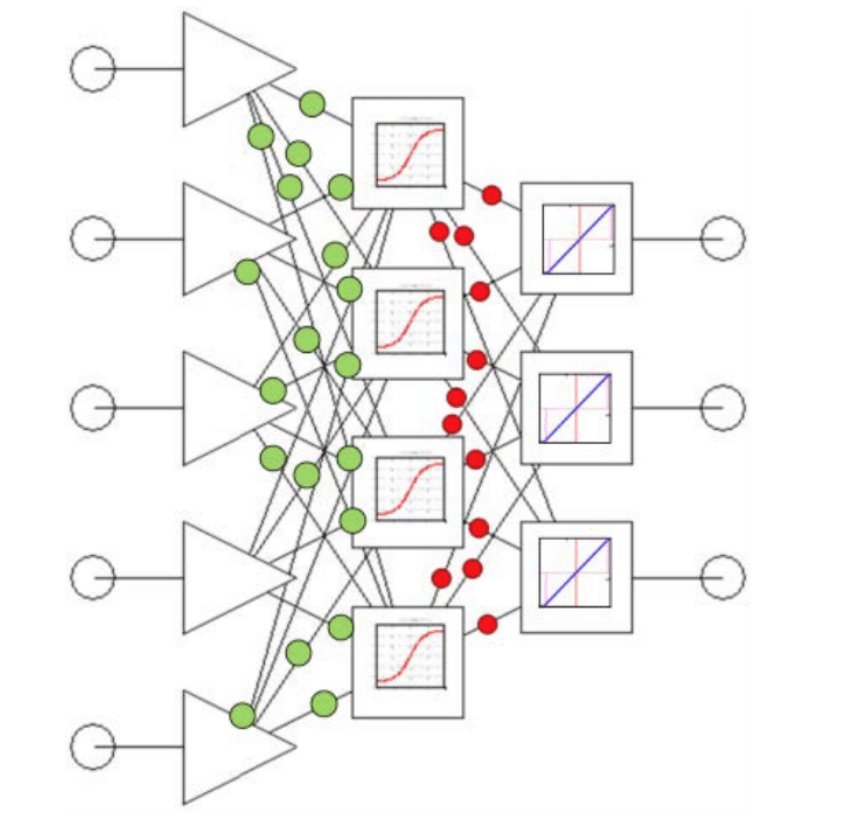
\includegraphics[width=0.5\linewidth]{img/MLP.jpg}}
  \caption{Schemat MLP.}
\end{figure}

\subsection{Neuron}

Podstawowy element budujący strukturę sieci neuronowej. Jest to element przetwarzający
informacje, w pewnym stopniu wzorowany na funkcjonowaniu biologicznej komórki nerwowej,
ale bardzo uproszczony.

Z powodu tych uproszczeń w  zasadzie nie powinno się używać dla tych elementów nazwy ‘neuron’,
bo ich właściwości daleko odbiegają od prawdziwych komórek nerwowych i ich dokładnych modeli
(na przykład dostępnych w programie GENESIS). Ale nazwa neuron przy-jęła się i jest
powszechnie używana.

W strukturze neuronu odnaleźć można wiele wejść oraz jedno wyjście. Ważnym składnikiem
neuronu jest komplet wag, których wartości decydujące o zachowaniu neuronu zazwyczaj
ustalane są w trakcie procesu uczenia.

\begin{figure}[h]
  \centering
  \fbox{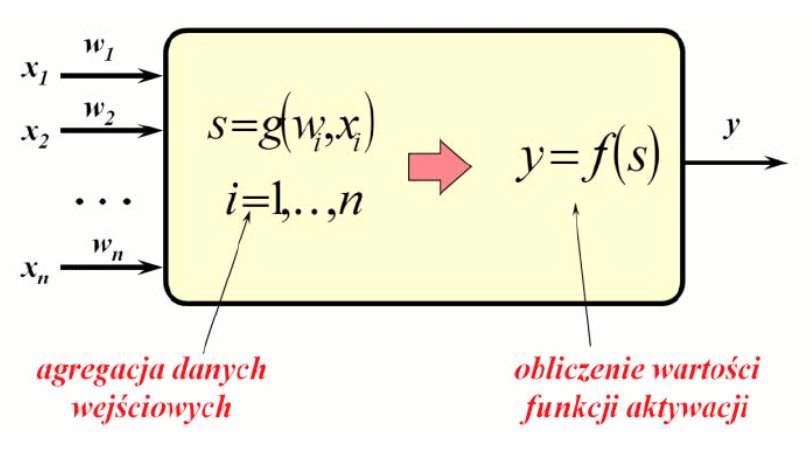
\includegraphics[width=0.5\linewidth]{img/neuron.jpg}}
  \caption{Schemat neuronu}
\end{figure}

W  neuronie wykonywane są zwykle dwie czynności: agregacja danych wejściowych
(z  uwzględnieniem  wag) oraz generacja sygnału wyjściowego (danej wyjściowej).
Ze względu na sposób agregacji oraz formę funkcji aktywacji wyróżnia się różne typy
neuronów. Najczęściej stosowane są neurony liniowe, neurony sigmoidalne i neurony radialne.
Odmianą neuronów sigmoidalnych są neurony tangensoidalne.[1]s

\subsection{Neuron sigmoidalny}

Jest to najbardziej popularny neuron nieliniowy, nadający się do budowy sieci MLP.
W neu-ronie sigmoidalnym zastosowana jest liniowa agregacja danych wejściowych
(często z  uwzględnieniem składnika BIAS) oraz sigmoidalna funkcja aktywacji.
Na marginesie można dodać, że schemat działania neuronu sigmoidalnego jest najbardziej
zbliżony do działania prawdziwej biologicznej komórki nerwowej.

\begin{figure}[h]
  \centering
  \fbox{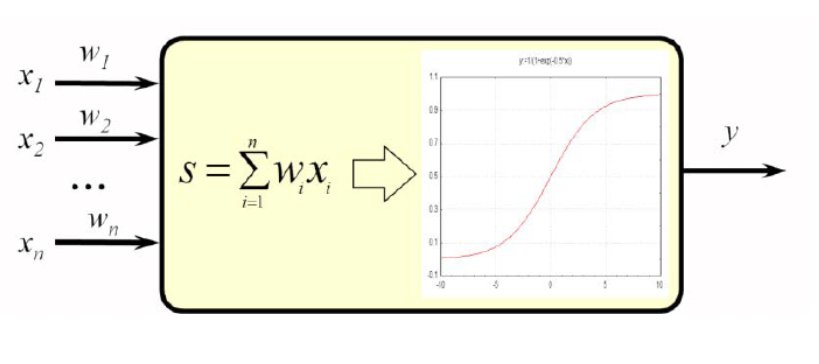
\includegraphics[width=0.5\linewidth]{img/neuronSigm.jpg}}
  \caption{Schemat neuronu sigmoidalnego}
\end{figure}

Warto jeszcze raz podkreślić, że zdecydowana większość dobrze funkcjonujących sieci neuronowych,
wykorzystywanych w praktyce w różnych dziedzinach. wykorzystuje w swojej strukturze,
a zwłaszcza w warstwach ukrytych, składniki w postaci neuronów sigmoidalnych.

\subsection{Perceptron}

Nazwa kojarzona często z jednokierunkowymi sieciami neuronowymi uczonymi metodą uczenia z nauczycielem.
Nazwa ta została po raz pierwszy użyta dla określenia sprzę-towej elektromechanicznej sieci neuronowej,
którą zbudował i przebadał  w 1960 roku Frank Rosenblatt na Uniwersytecie Cornella.

\subsection{Epoka}

Podczas uczenia sieci neuronowej trzeba wykonać bardzo wiele kroków algorytmu uczenia zanim błąd
stanie się akceptowalnie mały. Tymczasem zbiór uczący zawiera zwykle ograniczoną liczbę przypadków
uczących, w typowych przypadkach setki lub nawet tysiące razy mniej liczną niż liczba
koniecznych kroków algorytmu uczenia. Z tego zestawienia wynika, że zbiór uczący musi
być wykorzystywany w procesie uczenia wielokrotnie. Dla zaznaczenia tego faktu wprowadzono
pojęcie epoki, rozumiejąc pod tym pojęciem jednorazowe użycie w procesie uczenia wszystkich
przypadków uczących zawartych w zbiorze uczącym. Po wykonaniu wszystkich kroków należących
do jednej epoki algorytm uczący dokonuje oceny zdolności sieci do generalizacji wyników
uczenia przy wykorzystaniu zbioru walidacyjnego. Po stwierdzeniu, że zarówno błąd obliczany
na zbiorze uczącym, jak i błąd wyznaczony dla zbioru walidacyjnego nadal jeszcze obiecująco
maleją – algorytm uczący wykonuje następną epokę. W przeciwnym przypadku proces uczenia
zostaje zatrzymany.

Gdyby w  kolejnych epokach przypadki uczące pokazywać stale w tej samej
kolejności – to istniałaby obawa, że proces uczenia może zmieniać wagi w kółko,
powracając po każ-dym cyklu do punktu wyjścia. Przedstawia to rysunek, na którym
po lewej stronie pokazano właśnie taki „zapętlony” proces zmiany wag, nie prowadzący
do nauczenia sieci nawet po bardzo długim procesie uczenia. Na rysunku pokazano cykliczne
zmienianie się wartości dwóch wybranych wag (bo tylko to można pokazać na rysunku),
ale podobny niekorzystny proces zachodzi także dla wszystkich innych wag w całej sieci.

Zapętleniu uczenia można zapobiec poprzez randomizację zbioru uczącego,
to znaczy poprzez zmianę kolejności pokazywania poszczególnych przypadków uczących
w kolejnych epokach. Wtedy proces zmiany wag w trakcie uczenia porządkuje się i wyraźnie widać,
że zmierza do okre-ślonego celu, odpowiadającego optymalnemu zestawowi wag zapewniającemu 
rozwiązywanie stawianych sieci zadań z minimalnym błędem (co pokazano na rysunku po prawej stronie).

\subsection{Jednokierunkowa sieć neuronowa}

Sieci neuronowe budowane są zazwyczaj w taki sposób, że przepływ sygnałów odbywa się
w nich wyłącznie w kierunku od wejścia (poprzez ewentualne warstwy ukryte) do wyjścia.
Wykluczony jest przepływ sygnałów w drugą stronę, co powoduje, że sieci tego typu są
przeciwstawiane sieciom rekurencyjnym. Sieci spełniające wyżej podany warunek nazywane
są sieciami jednokierunkowymi albo sieciami typu feedforward. Sam przepływ sygnałów w
jednym kierunku (od wejścia do wyjścia) nie przesądza jeszcze o rodzaju sieci i zasadzie 
jej działania, gdyż wśród jednokierunkowych sieci neuronowych wyróżnić można między
innymi wielowarstwowe perceptrony (sieci MLP), sieci radialne (RBF), sieci uogólnionej
regresji (GRNN), probabilistyczne sieci neuronowe (PNN) i inne. W praktyce autorzy
najczęściej utożsamiają nazwę sieci jednokierunkowej z siecią typu MLP.

\subsection{Funkcja aktywacji}

Po agregacji danych wejściowych z uwzględnieniem wag powstaje sygnał sumarycznego pobudzenia.
Rola funkcji aktywacji polega na tym, że musi ona określić sposób oblicza-nia wartości
sygnału wyjściowego neuronu na podstawie wartości tego sumarycznego pobudzenia.
W literaturze rozważano wiele różnych propozycji funkcji aktywacji,
jednak do powszechnego użytku weszły właściwie cztery z  nich: funkcja liniowa (neuron liniowy),
funkcja sigmoidalna (neuron sigmoidalny), funkcja tangensoidalna (dokładnie jest to funkcja
tangens hiperboliczny, ale skrótowo mówi się właśnie neuron tangensoidalny) oraz funkcja
Gaussa (neuron radialny).

\subsection{Funkcja błędu}

Błąd popełniany przez sieć neuronową zależny jest od współczynników wag występujących
w sieci i doskonalonych przez algorytmy uczenia. Jeśli wyobrazimy sobie (patrz rysunek),
że w danym momencie procesu uczenia w sieci został ustalony pewien zestaw wag
(nazwany na rysunku pierwszym zestawem) i jeśli przy tym zestawie wag przeprowadzimy
egzamin, to uzyskamy pewną wartość błędu, przedstawioną na rysunku przy pomocy pionowej
strzałki. Jeśli wartość zestawu wag się zmieni (na przykład w wyniku uczenia)
i będziemy mieli do czynienia z drugim zestawem – to dla niego także można będzie
wyznaczyć błąd i przedstawić go – jak na rysunku – przy pomocy niższej strzałki.
Jeśli taką czynność wystawiania pionowych strzałek oznaczających wartości błędów
wykonamy w każdym punkcie szarej płaszczyzny, re-prezentującej na rysunku wszystkie
możliwe zestawy wag – to wierzchołki strzałek wyznaczą pewną powierzchnię rozpiętą ponad
szarą płaszczyzną. Właśnie ta powierzchnia to potrzebna do wielu celów (między innymi
w opisie procesu uczenia) funkcja błędu.

\subsection{Wagi}

Parametry neuronu decydujące o jego właściwościach i roli w procesie
rozwiązywania przez sieć postawionego zadania. Zwykle wagi dopasowuje
w całej sieci używany algorytm ucze-nia lub samouczenia.
Komplet wartości wag ustalonych we wszystkich neuronach w trakcie uczenia
lub samouczenia determinuje wiedzę, jaką posiada sieć neuronowa.

\section{Omówienie wykorzystanej technologii, danych oraz zbudowanej sieci}

W pracy wykorzystany zostanie framework do głębokiego uczenia o nazwie TensorFlow,
a badanymi danymi będą obrazy cifar10.

\begin{figure}[h]
  \centering
  \fbox{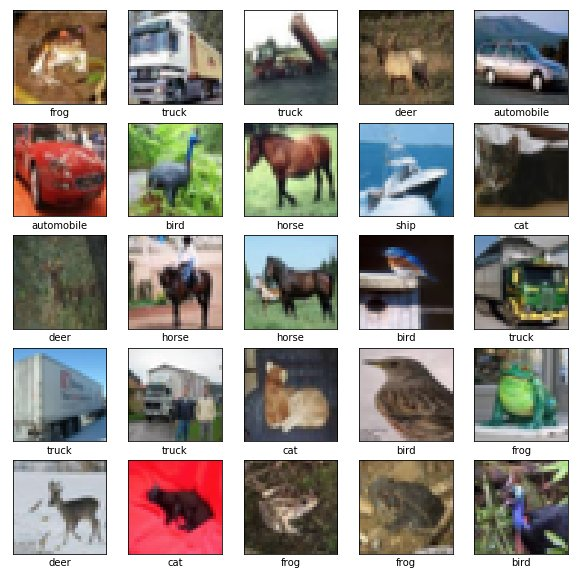
\includegraphics[width=0.5\linewidth]{img/cifar.jpg}}
  \caption{Schemat neuronu sigmoidalnego}
\end{figure}

Jak widać obrazy cifar przedstawiają różne zwierzęta, samochody i inne. Są one odpowiednio skategoryzowane.
Podstatowawą sięcią neuronową wykorzystywaną do tego zadania jest sieć trzy warstwowa.

Rząd neuronów nazywa się warstwą, a jedna sieć może mieć wiele warstw.
Architektura neuronów w sieci jest często nazywana topologią sieci.

Składa się z następujących warstw:
\subsection{Warstwa wejściowa}

Dolna warstwa, która pobiera dane z zestawu danych, nazywa się warstwą widoczną,
ponieważ jest odsłoniętą częścią sieci. Często sieć neuronowa jest rysowana
z widoczną warstwą z jednym neuronem na wartość wejściową lub kolumnę
w zbiorze danych. Nie są to neurony, jak opisano powyżej, ale po prostu
przekazują wartość wejściową do następnej warstwy.
W naszym przypadku jest to warstwa spłaszczająca,
sprawiająca że macierz jest przekształcana w wektor.

\subsection{Warstwa ukryta}

Warstwy po warstwie wejściowej są nazywane warstwami ukrytymi,
ponieważ nie są bezpośrednio narażone na dane wejściowe.
Najprostszą strukturą sieci jest posiadanie jednego neuronu w ukrytej warstwie,
który bezpośrednio wyprowadza wartość.

Biorąc pod uwagę wzrost mocy obliczeniowej i wydajnych bibliotek,
można zbudować bardzo głębokie sieci neuronowe. Głębokie uczenie się może odnosić się
do posiadania wielu ukrytych warstw w sieci neuronowej. Są głębokie, ponieważ byłyby
niewyobrażalnie powolne, aby trenować historycznie, ale mogą zająć sekundy lub minuty,
aby trenować przy użyciu nowoczesnych technik i sprzętu.

\subsection{Warstwa wyjściowa}

Ostatnia ukryta warstwa nazywana jest warstwą wyjściową i odpowiada za wyprowadzenie
wartości lub wektora wartości odpowiadających formatowi wymaganemu dla problemu.

Wybór funkcji aktywacji w warstwie wyjściowej jest silnie ograniczony przez typ problemu,
który modelujesz. Na przykład:

\begin{itemize}
  \item Problem regresji może mieć pojedynczy neuron wyjściowy, a neuron może nie mieć funkcji aktywacji.
  \item Problem z klasyfikacją binarną może mieć pojedynczy neuron wyjściowy i użyć funkcji
  aktywacji sigmoidalnej do wygenerowania wartości z zakresu od 0 do 1 w celu przedstawienia
  prawdopodobieństwa przewidywania wartości dla klasy 1. Można to zmienić w wyraźną wartość
  klasy za pomocą progu 0,5 i wartości przyciągania mniejsze niż próg do 0, w przeciwnym razie do 1.
  \item Problem klasyfikacji wielu klas może mieć wiele neuronów w warstwie wyjściowej,
  po jednym dla każdej klasy (np. Trzy neurony dla trzech klas w znanym problemie
  klasyfikacji kwiatów tęczówki). W takim przypadku można zastosować funkcję aktywacji
  softmax do wyprowadzenia prawdopodobieństwa sieci przewidującego każdą
  z wartości klasy. Wybierając wyjście z najwyższym prawdopodobieństwem,
  można wykorzystać do uzyskania wyraźnej wartości klasyfikacji klasy.
\end{itemize}

\subsection{Funkcja optymalizacyjna}

Jest to procedura poszukiwania minimum globalnego funkcji błędu.
Jedną ze znanych metod jest tzw. momentum, czyli funkcji pochodnej biorącej pod uwagę poprzedni
znak pochodnej.
Standardowym podejściem jest funkcja gradientu. Znajdowanie minimum globalnego nie jest łatwym zadaniem.

\section{Badania}

Nasz model w tensorflow jest trzywarstwowy i wygląda tak:
\begin{lstlisting}
model = tf.keras.models.Sequential([
    layers.Flatten(input_shape=(32,32,3)),
    layers.Dense(1024, activation='relu', use_bias=True),
    layers.Dense(10, activation='softmax', use_bias=True)
])
\end{lstlisting}

Jak widać jest to najprostrza sieć trzywarstwowa z funkcją aktywacyjną softmax dla wyjściowej
warstwy oraz biasem. A więc nadaje się do problemu wieloklasowego.

\begin{figure}[h]
  \centering
  \fbox{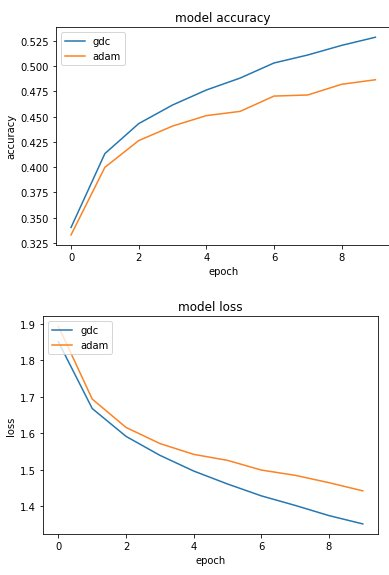
\includegraphics[width=0.5\linewidth]{img/adam_vs_gdc.jpg}}
  \caption{Porównannie wyniku działania sieci przez 10 epok z innym algorytmem optymalizacji}
\end{figure}

Jak widać metoda gdc, która w tensorflow korazysta z momentum okazała się być lepsza niż metoda adam.
Skoro wiemy, że optymalizacja oparta na momentum jest lepsza od optymalizacji adam, spróbójmy inaczej
poleprzyć naszą metodę dodając do niej kolejną warstwę.

\begin{figure}[H]
  \centering
  \fbox{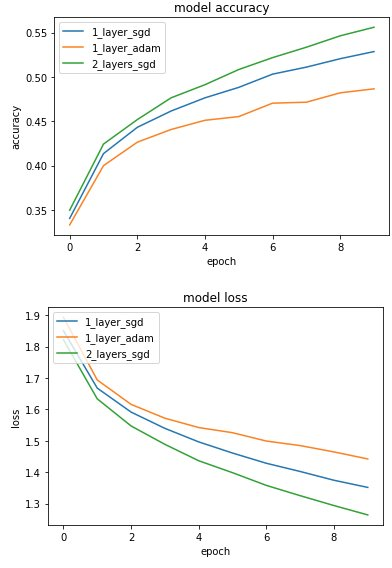
\includegraphics[width=0.5\linewidth]{img/2layers.jpg}}
  \caption{Porównannie wyniku działania sieci przez 10 epok
  z innym algorytmem optymalizacji oraz dodatkową warstwą ukrytą.}
\end{figure}

Jak widać po rysunku zastosowanie dodatkowej warstwy rzeczywiście poprawiło wynik,
jednak należy pamiętać, że wydłuża ona uczenie się algorytmu.
Zobaczmy jaka będzie skuteczność po dodaniu trzeciej warstwy ukrytej.

\begin{figure}[H]
  \centering
  \fbox{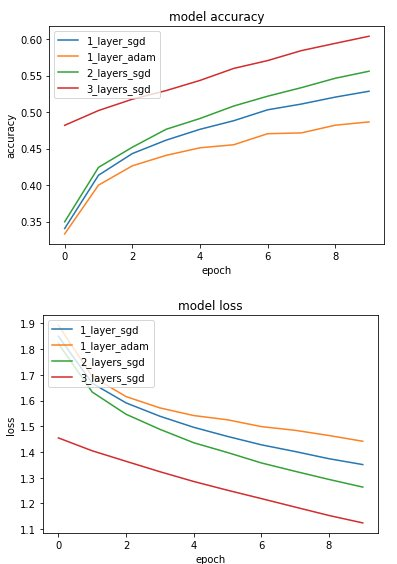
\includegraphics[width=0.5\linewidth]{img/3layers.jpg}}
  \caption{Porównannie wyniku działania sieci przez 10 epok
  z innym algorytmem optymalizacji oraz dodatkową trzecia warstwą ukrytą.}
\end{figure}

Wykres ten pokazuje, że nie tylko trzecia warstwa wpływa na wynik, ale także dobór wag początkowych dla algorytmu,
bo jak widać wykres sieci z trzema warstwami ukrytymi ma większe wyniki na początek, co znaczy, że miał wylosowane lepsze wagi.

\begin{figure}[H]
  \centering
  \fbox{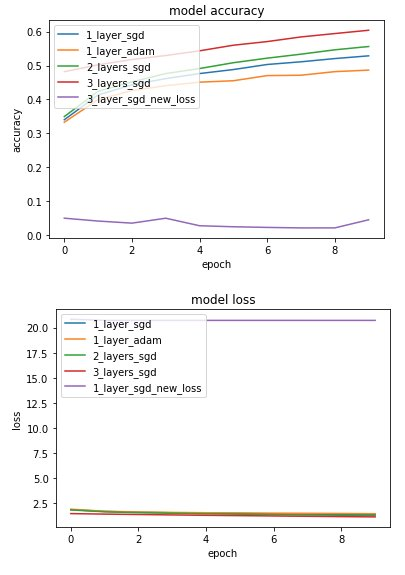
\includegraphics[width=0.5\linewidth]{img/loss.jpg}}
  \caption{Porównannie wyniku działania sieci przez 10 epok
  z innym algorytmem optymalizacji oraz inną funkcją straty.}
\end{figure}

Ten wykres pokazuje natomiast, że w algorytmie musi być odpowiednio dobrana funkcja straty do problemu.
W najgorszej sieci skorzystałem z funkcji straty obliczającą utratę 
dywergencji Kullbacka-Leiblera między wartością przewidywaną a prawdziwą.
Ta funkja straty dała fatalne rezultaty.

Podsumowując, wyniki sieci neuronowej zależą od wylosowanych wag sieci, funkcji straty, funkcji optymalizacyjnej oraz liczb warstw sieci.
Zależą także od funkcji aktywacyjnej danych warstw sieci neuronowej.

\section*{References}

\small

[1] Maciej Szaleniec \ \& Ryszard Tadeusiewicz\ LEKSYKON SIECI NEURONOWYCH 
[Lexicon on Neural Networks] \ Projekt nauka \ 978-83-63270-10-0.

\end{document}

Poni¿ej znajduje siê tabela, w której znajduj¹ siê informacje jak zapisaæ poprawnie polskie znaki w formie zakodowanej:
POLSKA LITERA   KOD TEX POLSKA LITERA   KOD TEX
¹       \k{a}   ¥       \k{A}
æ       \'c     Æ       \'C
ê       \k{e}   Ê       \k{E}
³       \l{}    £       \L{}
ñ       \'n     Ñ       \'N
ó       \'o     Ó       \'O
œ       \'s     Œ       \'S
¿       \.z     ¯       \.Z
Ÿ       \'z            \'Z

